\section{Recovering parameters}
\label{sec:undirected}

% Transition
We have thus far shown how to recover the conditional moments
$\mOpp{v}{i} = \BP(x_v \mid h_i)$ for each exclusive view $x_v$ of each hidden variable $h_i$,
as well as the hidden marginals $Z_S = \BP(\vh_S)$ for each bidependent subset of hidden variables $S$.
Now all that remains to be done is to recover the parameters.

Since our graphical model is in canonical form (\assumptionref{canonical}),
all cliques $\sC \in \sG$
either consist of hidden variables $\vh_\sC$ or are of the form $\{x_v,h_i\}$.
The key observation is that the clique marginals are actually sufficient
statistics of the model $p_\theta$.
How we turn these clique marginals $\{ \Pr(\bx_\sC,\bh_\sC) \}_{\sC \in \sG}$
into parameters $\theta$ depends on the exact model parametrization.

For directed models, the parameters are simply the local conditional tables
$p_\theta(a \mid \Pa(a))$ for each clique $\sC = \{a\} \cup \Pa(a)$.
These conditional distributions can be obtained by simply normalizing $Z_\sC$
for each assignment of $\Pa(a)$.

%by relating the recovered conditional moments with the expected features of
%the log-linear model.

% Define model
%As before, let $\sG$ be a graphical model with observed variables $\bx$ and hidden variables $\bh$
%(see \figureref{examples-mrf} for an example).
%For each clique $\sC \in \sG$, we have a feature vector $\phi_\sC(\vx_\sC, \vh_\sC)$,
%where $\vx_\sC$ and $\vh_\sC$ are the observed and hidden variables in $\sC$, respectively.
%Let $\phi(\vx, \vh) = \sum_{\sC \in \sG} \theta^\top \phi_\sC(\vx_\sC,\vh_\sC)$ be the global feature vector.
%We consider log-linear models of the following form:
%\begin{align*}
%p_\theta(\vx, \vh) &= \exp\left( \theta^\top \phi(\vx,\vh) - A(\theta) \right),
%\end{align*}
%where $A(\theta) = \log \sum_{\vx, \vh}  \exp( \theta^\top \phi(\vx,\vh) )$ is the log-partition function.

% FIGURE: example
\begin{figure}
  \centering
  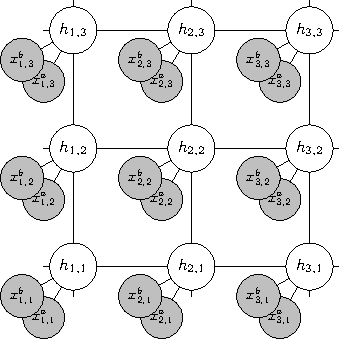
\includegraphics[width=0.6\columnwidth]{figures/mrf.pdf}
%  \subimport{figures/}{mrf.tikz}
  \caption{Example: undirected grid model where each hidden variable has two
  conditionally independent observations.
  This model has high treewidth,
  but we can estimate it efficiently using pseudolikelihood.}
  \label{fig:examples-mrf}
\end{figure}

%Of course, the log-likelihood is non-concave:
%\begin{align*}
  %L_\text{unsup}(\theta) \eqdef \E_{\vx \sim p_{\theta^*}}[\log \sum_{\vh \in \sH} p_\theta(\vx,\vh)],
%\end{align*}
%where we are assuming for simplicity that we have infinite data drawn from the true distribution $p_{\theta^*}$.
For undirected log-linear models, the canonical parameters $\theta$ cannot be obtained locally,
but we can construct a global convex optimization problem to solve for $\theta$.
Suppose we were able to observe $\vh$.
Then we could optimize the \emph{supervised} likelihood, which is concave:
\begin{align}
  L_\text{sup}(\theta)
  & \eqdef \E_{(\vx,\vh) \sim p_{\theta^*}}[\log p_\theta(\vx,\vh)] \nonumber \\
  & = \theta^\top \left(\sum_{\sC \in \sG} \E[\phi(\vx_\sC,\vh_\sC)]\right) - A(\theta).
\label{eqn:logLinearSupervised}
\end{align}
Of course we don't have supervised data,
but we do have the marginals $\Pr(\vx_\sC,\vh_\sC)$,
from which we can easily compute the expected features:
%recall that the method of moments provides the hidden marginals $Z_\sC = \BP(\vh_\sC)$
%and conditional moments $\mOpp{v}{i} = \Pr(x_v \mid h_i)$.
%Assuming our graphical model is in canonical form (\lemmaref{reduction}),
%every observed variable is connected to exactly one hidden variable.
%Then $Z_\sC$ and $\mOpp{v}{i}$ directly yield marginals for every clique $\BP(\vx_\sC, \vh_\sC)$.
%Given these marginals, we can compute the expected local feature vector:
\begin{align}
\label{eqn:logLinearFeatures}
\mu_\sC \eqdef \E[\phi(\vx_\sC,\vh_\sC)] = \sum_{\vx_\sC,\vh_\sC} \BP(\vx_\sC,\vh_\sC) \phi(\vx_\sC,\vh_\sC).
\end{align}
%Note that $\{\mu_\sC\}_{\sC \in \sG}$ are exactly the sufficient statistics of the model (\equationref{logLinearSupervised}),
Therefore, we can optimize the supervised likelihood objective without actually
having any supervised data!
In the finite data regime, the method of moments yields the estimate
$\hat \mu^\text{mom}_\sC$ which approximates the true $\mu_\sC$.
In supervised learning, we obtain a different estimate $\hat\mu^\text{sup}_\sC$ of $\mu_\sC$ based on an empirical average
over data points.
In the limit of infinite data, both estimators converge to $\mu_\sC$.

%\algorithmref{undirected} summarizes our approach.
%In \sectionref{exclusiveViews}, we showed that $\LearnMarginals$ is a consistent
%estimator for $Z_\sC$ for any bottlenecked clique in the graphical model. 
%Consequently, \algorithmref{undirected}
%is also a consistent estimator.\footnote{Of course, the log-linear model must be identifiable.
%Identifability is violated, for example, if two components of $\phi(\vx_\sC, \vh_\sC)$ were identical.
%In general, we can identify the parameters up to the kernel of $\nabla^2 A(\theta)$.}

%\renewcommand{\algorithmicrequire}{\textbf{Input:}}
%\renewcommand{\algorithmicensure}{\textbf{Output:}}
\begin{algorithm}
  \caption{\LearnParameters}
  \label{algo:undirected}
  \begin{algorithmic}
    \REQUIRE Conditional moments $\mOpp{v}{i} = \Pr(x_v \mid h_i)$
             and hidden marginals $Z_S = \Pr(\bh_S)$.
    \ENSURE Parameters $\theta$.
    \IF{$\sG$ is directed} \STATE Normalize $\Pr(a,\Pa(a))$ for $a \in \bx \cup \bh$.
    \ELSIF{$\sG$ is undirected with low treewidth}
      \STATE Compute features $\mu_\sC$ for $\sC \in \sG$ (\equationref{logLinearFeatures}).
      \STATE Optimize full likelihood (\equationref{logLinearSupervised}).
    \ELSIF{$\sG$ is undirected with high treewidth}
      %\STATE Compute expected features $\mu_{\{a\} \cup B}$ for $a \in \bh, B \in \sB(a)$ (\equationref{neighborhoodFeatures}).
      \STATE Compute features $\mu_{\{a\} \cup \sN(a)}$ for $a \in \bh$ (\equationref{neighborhoodFeatures}).
      \STATE Optimize pseudolikelihood (\equationref{pseudolikelihood}).
    \ENDIF
    \end{algorithmic}
\end{algorithm}

% Learning with partial moment constraints
\paragraph{Remark} If we have exclusive views for only a subset of the cliques,
we can still obtain the expected features $\mu_\sC$ for those cliques
  and use posterior regularization \citep{graca08em}, measurements \citep{liang09measurements}, or generalized
  expectation criteria \citep{mann08ge}
  to encourage $\E_{p_\theta}[\phi(\vx_\sC,\vh_\sC)]$ to match $\mu_\sC$.
The resulting objective functions would be non-convex, but we expect
  local optima to be less of an issue.
  %How to characterize this precisely is an interesting direction for future work.

%%%%%%%%%%%%%%%%%%%%%%%%%%%%%%%%%%%%%%%%%%%%%%%%%%%%%%%%%%%%
\subsection{Pseudolikelihood}
\label{sec:pseudolikelihood}

While we now have a complete algorithm for estimating directed and undirected
models, optimizing the full likelihood (\equationref{logLinearSupervised})
can still be computationally intractable for undirected models with high treewidth
due to the intractability of the log-partition function $A(\theta)$.
One can employ various variational approximations of $A(\theta)$ \cite{wainwright08varinf},
but these generally lead to inconsistent estimates of $\theta$.
We thus turn to an older idea of pseudolikelihood \citep{besag75pseudo}.
The pseudolikelihood objective is a sum over the log-probability of each
variable $a$ given its neighbors $\sN(a)$:
\begin{align}
  \label{eqn:pseudolikelihood}
  L_\text{pseudo}(\theta) \eqdef \E_{(\bx,\bh) \sim p_{\theta^*}}\left[\sum_{a \in \bx \cup \bh} \log p_\theta(a \mid \sN(a))\right].
\end{align}
In the fully-supervised setting, it is well-known that pseudolikelihood
provides consistent estimates which are computationally efficient
but less statistically efficiency.\footnote{
Coincidentally, this is the same high-level motivation for using method of
moments in the first place.}

Let $\phi_{a,\sN(a)}(a, \sN(a)) = \sum_{\sC \ni a} \phi_\sC(\bx_\sC,\bh_\sC)$
denote the sum over cliques $\sC$ that contain $a$; note that $\phi_{a, \sN(a)}$ only depends on $a$ and its neighbors $\sN(a)$.
We can write each conditional log-likelihood from \equationref{pseudolikelihood} as:
\begin{align*}
p_\theta(a \mid \sN(a)) = \exp(\theta^\top\phi_{a,\sN(a)}(a, \sN(a)) - A_a(\theta; \sN(a))),
\end{align*}
where the conditional log-partition function $A_a(\theta; \sN(a)) = \log \sum_{a'} \exp(\theta^\top\phi_{a,\sN(a)}(a', \sN(a)))$
involves marginalizing only over the single variable $a$.

If we knew the marginals for each neighborhood,
\begin{align}
  \mu_{a,\sN(a)} &\eqdef \E[\phi_{a,\sN(a)}(a,\sN(a))], \label{eqn:neighborhoodFeatures}
\end{align}
then we would be able to optimize the pseudolikelihood objective again without
having access to any labeled data.
Unfortunately, $\{a\}\cup\sN(a)$ does not always have exclusive views.
For example, consider $a = h_1$ and $\sN(a) = \{h_2,h_3,h_4\}$ in \figureref{examples-tree}.

However, we can decompose $\{a\}\cup\sN(a)$ as follows:
conditioning on $a$ partitions $\sN(a)$ into independent subsets;
let $\sB(a)$ be the collection of these subsets,
which we will call \emph{sub-neighborhoods}.
For example, $\sB(h_1) = \{ \{h_2\},\{h_3\},\{h_4\} \}$ in \figureref{examples-tree}
and $\sB(h_{2,2}) = \{ \{ h_{1,2}, h_{2,3}, h_{3,2}, h_{2,1} \} \}$ contains a single sub-neighborhood in \figureref{examples-mrf}.

A key observation is that for each sub-neighborhood $B \in \sB(a)$, each $\{a\} \cup B$ is bidependent:
conditioning on $a$ does not introduce new independencies within $B$ by construction of $\sB(a)$,
and conditioning on any $b \in B$ does not either since every other $b' \in B \backslash \{b\}$
is connected to $a$.
Assuming $\sG$ is bottlenecked, by \lemmaref{bottleneck-views}
we have that $\{a\} \cup B$ has exclusive views.
Hence, we can recover $\Pr(a,B)$ for each $a$ and $B \in \sB(a)$.
Based on conditional independence of the sub-neighborhoods $B$ given $a$,
we have that $\Pr(a, \sN(a)) = \Pr(a) \prod_{B \in \sB(a)} \Pr(B \mid a)$.
This allows us to compute the expected features $\mu_{a,\sN(a)}$ and use them
in the optimization of the pseudolikelihood objective.

%  Therefore, we can adapt our algorithm ($\LearnMarginals$) to estimate all
%  marginals of the form $Z_{a,\sN(a)} \eqdef \Pr(a,\sN(a))$,
%  from which we can compute the features $\mu_{a,\sN(a)}$,
%  and optimize \equationref{pseudolikelihood} to obtain a consistent estimate of $\theta$.

Note that our pseudolikelihood-based approach
does depend exponentially on the size of the sub-neighborhoods,
which could be exceed the largest clique size.
Therefore,
%for our approach to be effective,
each node essentially should have low degree or locally exhibit a lot of
conditional independence.
%While this method is only viable for graphs with small sub-neighboof low
%degree, i.e.\@ when $|\sN(a)|$ is small,
On the positive side, we can handle graphical models with high treewidth;
neither sample nor computational complexity necessarily depends on the treewidth.
%For example, for an $n \times n$ grid model, the treewidth is $n$,
%but it is the degree (only 4 in this case) that governs the computational complexity.
For example, an $n\times n$ grid model has a treewidth of $n$, but the degree is at most $4$.
